\section{System Model}
%----------------------------------------------------------------------------------------%
\subsection{Network Model}
We consider an edge computing system with $K$ Access Points (APs) and $M$ edge servers, which are connected in a network as illustrated in Fig.\ref{fig:system}.
Denote the sets of APs and edge servers as $\apSet \define \set{1,\dots,K}$ and $\esSet \define \set{1,\dots,M}$, respectively.
Each AP collects the computation jobs from the mobile users within its coverage, and makes decision for each job on which edge server it should be dispatched to.
\accept{In this paper, we shall focus on the dispatcher design at each AP.}
% We denote as $\apSet \define \set{1,\dots,K}$ and $\mathcal{M} \define \set{1,\dots,M}$ Access Points (AP) and Edge Servers (ES) respectively in our system, as depicted in Fig. \ref{fig:system}.

\begin{figure}[ht]
    \centering
    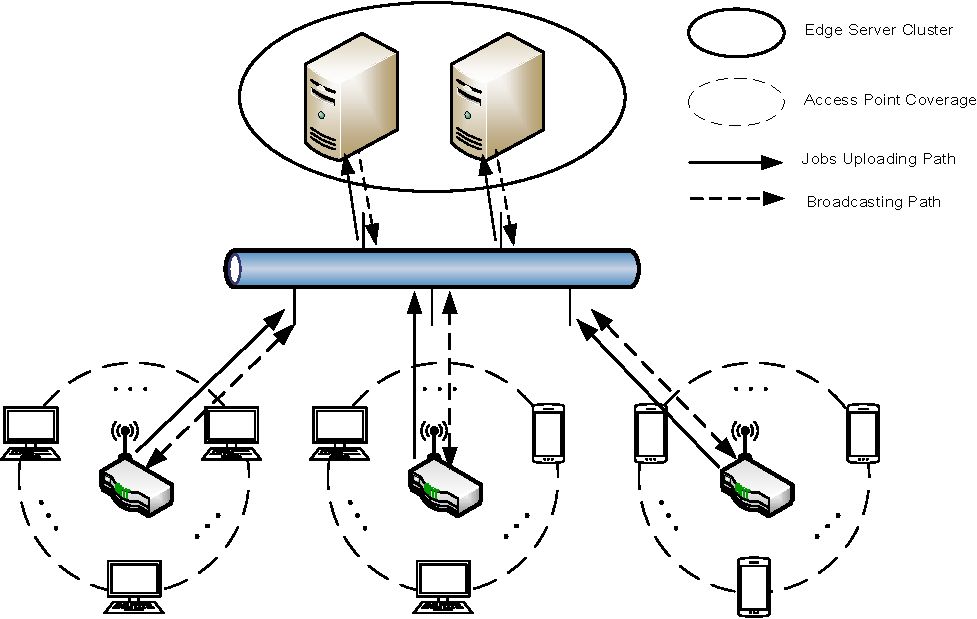
\includegraphics[width=0.45\textwidth]{system-model.pdf}
    \caption{The Illustration of MEC System Model}
    \label{fig:system}
\end{figure}

%NOTE: [job space support and arrival process]
The time axis of each AP is organized by time slots.
Without loss of generality, it is assumed that there are $J$ types of computation jobs supported in this system, which is denoted as $\jSpace \define \set{1,\dots,J}$.
The job arrivals in each time slot are modelled as independent Bernoulli distributions.
More specifically, the arrivals of the $j$-th type of jobs at the $k$-th AP are independent and identically distributed (i.i.d.) Bernoulli random variables, and the arrival probability is denoted as $\lambda_{k,j}$ ($\forall k\in\apSet, j\in\jSpace$).
% The User Equipment (UE) is connected to the AP and offload the computation jobs on demand to the AP. A list of types of jobs are supported on edge servers based on Virtual Machine (VM) resources, which is denoted as $\jSpace \define \set{1,\dots, J}$.
% which is obtained by statistics and denoted as $p_j \define \Pr\{\text{"j-type arrival"}\}$, where $\sum_{j\in\jSpace} p_j=1$.
% Thus the job arrival process on $k$-th AP ($\forall k\in\apSet$) is compounded of the job arrivals from all UE connected, which follows the assumption as follows.
% \begin{assumption}[Job Arrival Process for AP]
%     Thus average arrival rate of $j$-type jobs on $k$-th AP is $\mathbb{E}[A_{k,j}]=\lambda_{k,j}$.
% \end{assumption}


%NOTE: [uploading process]
Each AP then immediately dispatches each type of received jobs to one edge server.
Let $\omega_{k,j}$ denotes the index of edge server for the processing of the $j$-th types of jobs dispatched from the $k$-th AP ($\forall k\in\apSet, j\in\jSpace$).
Different types of jobs may have different distributions on the input data size.
Moreover, due to the random traffic in the network, the job uploading from one AP to one edge server consumes a random number of time slots.
\accept{
    It is assumed that the distributions of uploading delay of different jobs are independent and the job uploading are independnet among jobs.
    The uploading delay are i.i.d for all the $j$-th type of jobs from the $k$-th AP to the $m$-th edge server, which is denoted as $\mathcal{U}_{k,m,j}$ ranged in $(0,\Xi]$ with the unit of time slot ($\forall k\in\apSet, m\in\esSet, j\in\jSpace$).
}
In practice, the distribution of uploading delay may not be known to the APs or edge servers in advance.
% The AP itself is assumed with no computation capability, and thus the jobs are further dispatched to the edge servers for processing.
% The jobs on AP will be immediately dispatched to edge servers once arrives.
% The corresponding uploading time is \emph{un-predictable} over one AP-ES link, which is composed of \emph{communication delay} due to bandwidth available and propagation delay due to underlaid network.
% We assume that for $j$-type of job, the corresponding delay follows some distribution over one link from $k$-th AP to $m$-th ES ($\forall j\in\jSpace, k\in\apSet, \forall m\in\esSet$).

%NOTE: [processing process]
There are $J$ virtual machines (VMs) on one edge server for the computation of $J$ types of jobs.
For each type, the uploaded jobs are computed in a First-Come-First-Serve (FCFS) manner.
Furthermore, we adopt \emph{unrelated machines} assumption in \cite{tan-online} for job processing on edge servers, where the job processing time on different servers are machine dependent.
We denote $\mathcal{C}_{m,j}$ as the processing time distribution of $j$-th type job on the $m$-th edge serer, whose range is in $(0, c_{m,j}]$ with the unit of time slot ($\forall m\in\esSet, j\in\jSpace$).
The maximum job queue length for each VM is set as $l_Q$, which indicates that there are at most $l_Q$ jobs pending for one VM on the edge servers. \accept{The jobs submission over the limits would be rejected to the corresponding AP.}
% [abandon for \emph{unrelated machines model}]
% For convenience, we assign jobs with \emph{infinity} processing time when there are no  have no VM resource available with , and this kind of dispatching possibility will be rejected at the AP side.

\delete{We highlight the life cycle of the job being processed.}
%----------------------------------------------------------------------------------------%

\subsection{Periodic Broadcast of State Information}
%NOTE: 
Each AP forwards the computation jobs of different types to different edge servers.
In order to make dispatching decision, they should collect the state information from other APs and edge servers.
It is assumed that each AP and edge server broadcast their state information every $t_B$ time slots.

We firstly define the following notations on the state information.
\begin{itemize}
    \item the number of jobs in uploading;
        $R^{(k)}_{m,j,\xi}$ denotes the number of the $j$-th type of jobs been uploaded to the $m$-th edge servers $\xi$ time slots ago.
    \item the queueing state description for the $j$-th type jobs on the $m$-th edge server: $Q_{m,j} \define (L_{m,j}, \eta_{m,j})$, where:
    \begin{itemize}
        \item $L_{m,j}$ denotes the number of jobs in waiting;
        \item $\eta_{m,j}$ denotes the remaining time slots of the first job in processing;
    \end{itemize}
\end{itemize}

%NOTE: [State for AP and Edge Server]
The state information of one AP (say the $k$-th AP, $\forall k\in\apSet$) at the $i$-th broadcast are defined as follows.
\begin{align}
    \mathcal{R}_{k}(i) \define \set{R^{(k)}_{m,j,\xi}(i) | \forall m\in\esSet, j\in\jSpace, \xi \in [0,\Xi]}
\end{align}
Moreover, the state information of one edge server (say the $m$-th edge server, $\forall m\in\esSet$) at the $t$-th broadcast are defined as follows.
\begin{align}
    \mathcal{Q}_{m}(i) \define \set{Q_{m,j}(i) | \forall m\in\esSet, j\in\jSpace}
\end{align}

\delete{
    We further adopt the following time denotation.
    \begin{align}
        t_{i,n} = i \cdot T + n \cdot \tau, (i,n=0,1,2,\dots),
    \end{align}
    where $t_{i,n}$ denotes the $n$-th time slot in $i$-th interval w.r.t the start point. Especially, we denote as $t_{i} \define t_{i,0}$ as the start point of each broadcasting interval, which is called \emph{broadcast point}.
}

Thus the composed broadcasting information at the $i$-th broadcast is denoted as:
\begin{align}
    \Obsv(i) \define
        \Brace{
            \mathcal{R}_{k}(i), \mathcal{Q}_{m}(i) | \forall k\in\apSet, m\in\esSet
        }.
\end{align}

As the broadcasting latency is random due to underlaid network, different AP nodes would receive whole broadcast information at different time slots in one broadcast period.
We call the caused delay \emph{update latency}, and denote the latency in the $i$-th broadcast period for the $k$-th AP ($\forall k\in\apSet$) as $D_{i,k}$.
% $k$-th AP receives the last partial information at $t_{i} + D_{k,t}$.
Due to the un-predictability of \emph{update latency}, $D_{i,k}$ for the $k$-th AP in the $i$-th period could not be known exactly by other APs. This implies that the explicit sharing about timing information is not impossible in the distributed system.
Moreover, we assume that the broadcast period is selected with a value that always larger than the corresponding \emph{update latency}, i.e. $t_B > \hat{D}_k$ ($\forall k\in\apSet$), where $\hat{D}_k$ is the upper bound for $D_{i,k}$ ($i=1,2,\dots$).

In the problem formulation section, we will show that we could come up with better policy aware of the randomness of latency, and improve AP's policy in an iterative way.
Furthermore, with the help of algorithm design we could prove that our improved policy is with analytical performance bound under MDP framework.

% In the decentralized system, a information sharing scheme is indispensable to guarantee a global-wise optimal policy than local greedy policy.
% However, frequent information exchange would always introduce heavy network burden and communication latency is also a severe issue which causes stale information collection. So, an efficient scheme is needed to alleviate the communication burden and aware of the stale information impact.
% In this article, the proposed sharing scheme leverage a common periodic broadcast which lasting for adjustable period $T \define N \times \tau$. More specifically, the broadcasting is applied in a loose synchronized way that all the nodes (including AP and ES) starts broadcasting at the same start and is received in that period due to the stochastic latency.

% And we notice that though $\mathcal{R}(t_{i,n})$ and $\mathcal{Q}(t_{i,n})$ also exists in each time slot, the observed information is only available at the start of each interval via broadcast. Thus the shared information is actually a uniform sampling of the whole process.

% [abandon, definition for update latency]
% We denote as $D^{(p)}_{k,k'}(t_i)$ the broadcast delay between $k'$-th AP and $k$-th AP ($\forall k,k'\in\apSet$), and $D^{(s)}_{k,m}(t_i)$ the broadcast delay between $m$-th edge server and $k$-th AP ($\forall k\in\apSet,\forall m\in\esSet$).
% Then we denote the latency for $k$-th AP receives broadcast information from other nodes (including all edge server nodes and other AP nodes) as \emph{Maximum Broadcast Latency}.
% \begin{definition}[Maximum Broadcast Latency]
%     The maximum broadcast latency is the time when AP receives whole broadcast information with respect to the broadcast point. For $k$-th AP ($\forall k\in\apSet$) the latency for $i$-th interval is given as follows.
%     \begin{align}
%         &D_{k}(t_i) \define \max\Paren{ \set{D^{(p)}_{k,k'}(t_i), D^{(s)}_{k,m}(t_i) |\forall k',k \in\apSet, \forall m\in\esSet} }
%     \end{align}
% \end{definition}

\delete{
    Due to the introduced periodic broadcasting design and the information receiving latency, this kind of system is inherent of the structure that decisions are always made with obsolete and partial information.
    This implies that: if any agents change its decision with respect to newly-arrival broadcast information, it will disturb other agents' decisions from cooperation due to different information of system states.
    Thus, it's unacceptable to update agents' policy only when the agents all come up with exactly same information.
}
%----------------------------------------------------------------------------------------%